To characterize the dimensionality of GPU power-domain attack signatures,
we apply principal component analysis (PCA) to the combined telemetry from
the oversubscription (\S\ref{sec:eval-oversub}) and contention-isolation
(\S\ref{sec:eval-contention}) experiments
($N{=}17{,}412$ samples, 7 standardized features).

\begin{table}[t]
\centering
\caption{PCA variance decomposition and dominant feature loadings.}
\label{tab:pca_variance}
\small
\begin{tabular}{clcc}
\toprule
\textbf{PC} & \textbf{Top Loadings} & \textbf{Var. (\%)} & \textbf{Cum. (\%)} \\
\midrule
PC1 & Current (A) (+0.49); Power (W) (+0.49); Voltage (V) (-0.48) & 52.1 & 52.1 \\
PC2 & Latency (ms) (+0.86); SM Clock (MHz) (-0.34); di/dt (A/s) (-0.31) & 15.2 & 67.4 \\
PC3 & di/dt (A/s) (+0.94); Latency (ms) (+0.35); Voltage (V) (-0.02) & 14.4 & 81.7 \\
\bottomrule
\end{tabular}
\end{table}


Table~\ref{tab:pca_variance} shows the variance decomposition.
Three components capture 81.7\% of the total variance, and five
suffice for 95\%.
PC1 (52.1\%) loads almost equally on power, current, and (inversely)
voltage---the trio that defines the power-domain state.
This confirms that the dominant axis of variation in the telemetry
is the power draw itself, which the attacker's duty-cycled kernel
directly manipulates.
PC2 (15.2\%) captures latency inflation and its inverse correlation
with clock frequency: when the attacker forces DVFS contention,
the governor reduces the SM clock, increasing victim kernel latency.
PC3 (14.4\%) isolates the transient current derivative ($di/dt$),
reflecting the rapid current swings caused by the attacker's
on/off modulation pattern.

Figure~\ref{fig:pca_scatter} projects all samples onto the PC1--PC2 plane.
In both experiments, attack samples (red) separate clearly from
baseline samples (blue), with non-overlapping 95\% confidence ellipses
along the PC1 axis.
The oversubscription panel shows attack clusters displaced rightward
(higher power/current) across all five clock-cap levels, while
the contention-isolation panel reveals that attack separation persists
under both fixed-clock and default (DVFS-governed) policies---confirming
that the signature is not an artifact of a single clock-management strategy.

\begin{figure}[t]
  \centering
  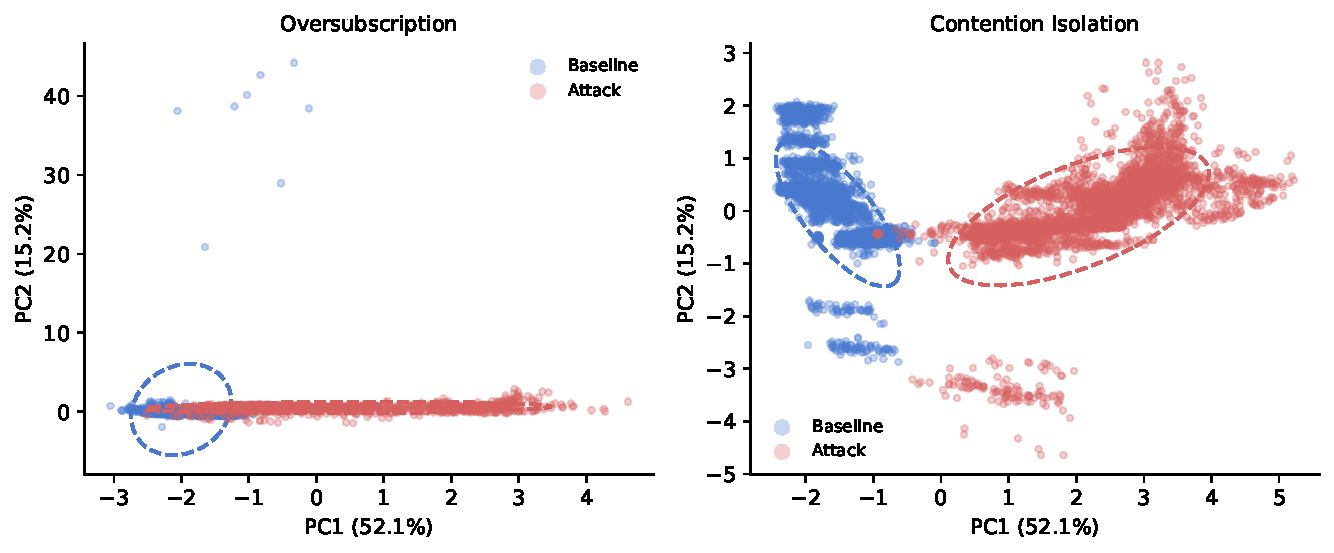
\includegraphics[width=\columnwidth]{figures/fig_pca_scatter.pdf}
  \caption{PC1 vs.\ PC2 projection of telemetry samples, colored by
    condition (blue = baseline, red = attack) with 95\% confidence
    ellipses.
    Left: oversubscription experiment (5 clock caps).
    Right: contention-isolation experiment (7 workloads $\times$ 2
    clock policies).}
  \label{fig:pca_scatter}
\end{figure}

\begin{figure}[t]
  \centering
  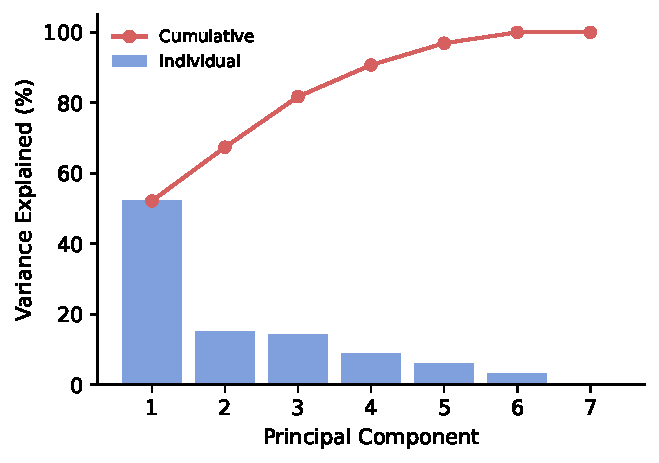
\includegraphics[width=0.65\columnwidth]{figures/fig_pca_scree.pdf}
  \caption{Scree plot showing individual and cumulative variance
    explained by each principal component.  Five components account
    for 96.9\% of total variance.}
  \label{fig:pca_scree}
\end{figure}

These results have two practical implications.
First, because a single component (PC1) captures over half the variance
and cleanly separates attack from baseline, a lightweight detector
can operate on a one-dimensional projection of the raw telemetry---no
high-dimensional classifier is required for initial triage.
Second, the loading structure reveals which sensors carry the most
discriminative information: power and current dominate PC1, while
clock frequency and latency dominate PC2.
A production monitoring stack can therefore prioritize these four
channels, reducing the bandwidth and storage cost of continuous
telemetry collection.
